\chapter{Introduction}\label{introduction}

% general flow: introduction of origin of nuclear theory -> structure of nucleus and nuclear matter -> problems of nuclear theory (how nuclei work, astrophysical applications (origin of elements), nucleus as a laboratory in the search for BSM physics, applications in national security, energy, medicine) -> explanation of past struggles with computational difficulty (phenom models) -> explanation that these models have low predictive power outside the domain in which they were fit -> need for better nuclear theory calculations in light of experimental advances in low-energy nuclear physics (FRIB) and astrophysics (LIGO results suggesting site of r-process) -> rapid expansion of range of calculations from first principles in recent years due to improvements in computational hardware and development of new computational methods -> focus on modern ab-initio methods (NCSM, IM-SRG, lattice QCD), RG methods, EFT methods -> use of these methods is state of the art in low-energy nuclear theory -> study of their correct, optimal application to calculations is an open problem


Nuclear theory is concerned with modeling atomic nuclei and nuclear matter. Nuclear matter is made of protons and neutrons, which are generally referred to as nucleons. Nucleons interact primarily through the strong interaction, which together with the weak interaction governs the stability of nuclear isotopes. Nuclear theory seeks to answer open questions in four areas: what are the properties of nuclei, especially exotic isotopes; what are the properties of nuclear matter in astrophysical systems such as neutron stars; what can be learned about beyond Standard Model (BSM) physics from the nucleus; and how can more accurate models of nuclear systems be leveraged in a variety of applications, ranging from national security and energy to medicine.

Nuclear theory faces two major challenges when trying to model systems of nucleons at low energies. The first is that this is a quantum many-body problem. Quantum many-body theory is relevant to many different fields, including quantum chemistry and condensed matter theory. Many-body problems quickly become intractable when approached naively due to the combinatorial growth of the size of the problem with respect to the number of particles. The second major challenge of nuclear theory is that while the forces between nuclei are given by quantum chromodynamics (QCD), the theory underlying the strong interaction, QCD cannot be solved in closed form at energies relevant to nuclei. The strong interaction is between quarks and gluons, collectively referred to as partons, which make up nucleons, instead of between nucleons themselves. In the past, these challenges forced nuclear physics to rely on phenomenological models, both for the form of the strong interaction and the treatment of the many-body problem. These models were typically fit to experimental data for certain nuclei and used to predict the properties of nearby nuclei. However, their predictive ability did not extend far outside the domain in which they were fit, limiting their range of applicability. Furthermore, they did not provide theorists with error estimates or any ways to tell when they became invalid.

With the Facility for Rare Isotope Beams (FRIB) on the horizon, there is demand for more accurate calculations of nuclear observables with new methods as well as for theoretical predictions of properties of heavy, exotic nuclei that have not been measured yet. Moreover, accurate models of nuclear matter are essential to understanding dense stars, supernovae, and certain astrophysical events, such as the collisions of neutron stars, which are hypothesized to be a location for the synthesis of heavy elements, such as gold and silver. Improved nuclear models are also essential in predicting the rate of certain nuclear decays, such as neutrino-less double-beta decay, which is currently being searched for by many experiments to answer whether or not neutrinos are Majorana particles, that is, they are their own anti-particle.

\begin{figure}[t]
    \begin{center}
        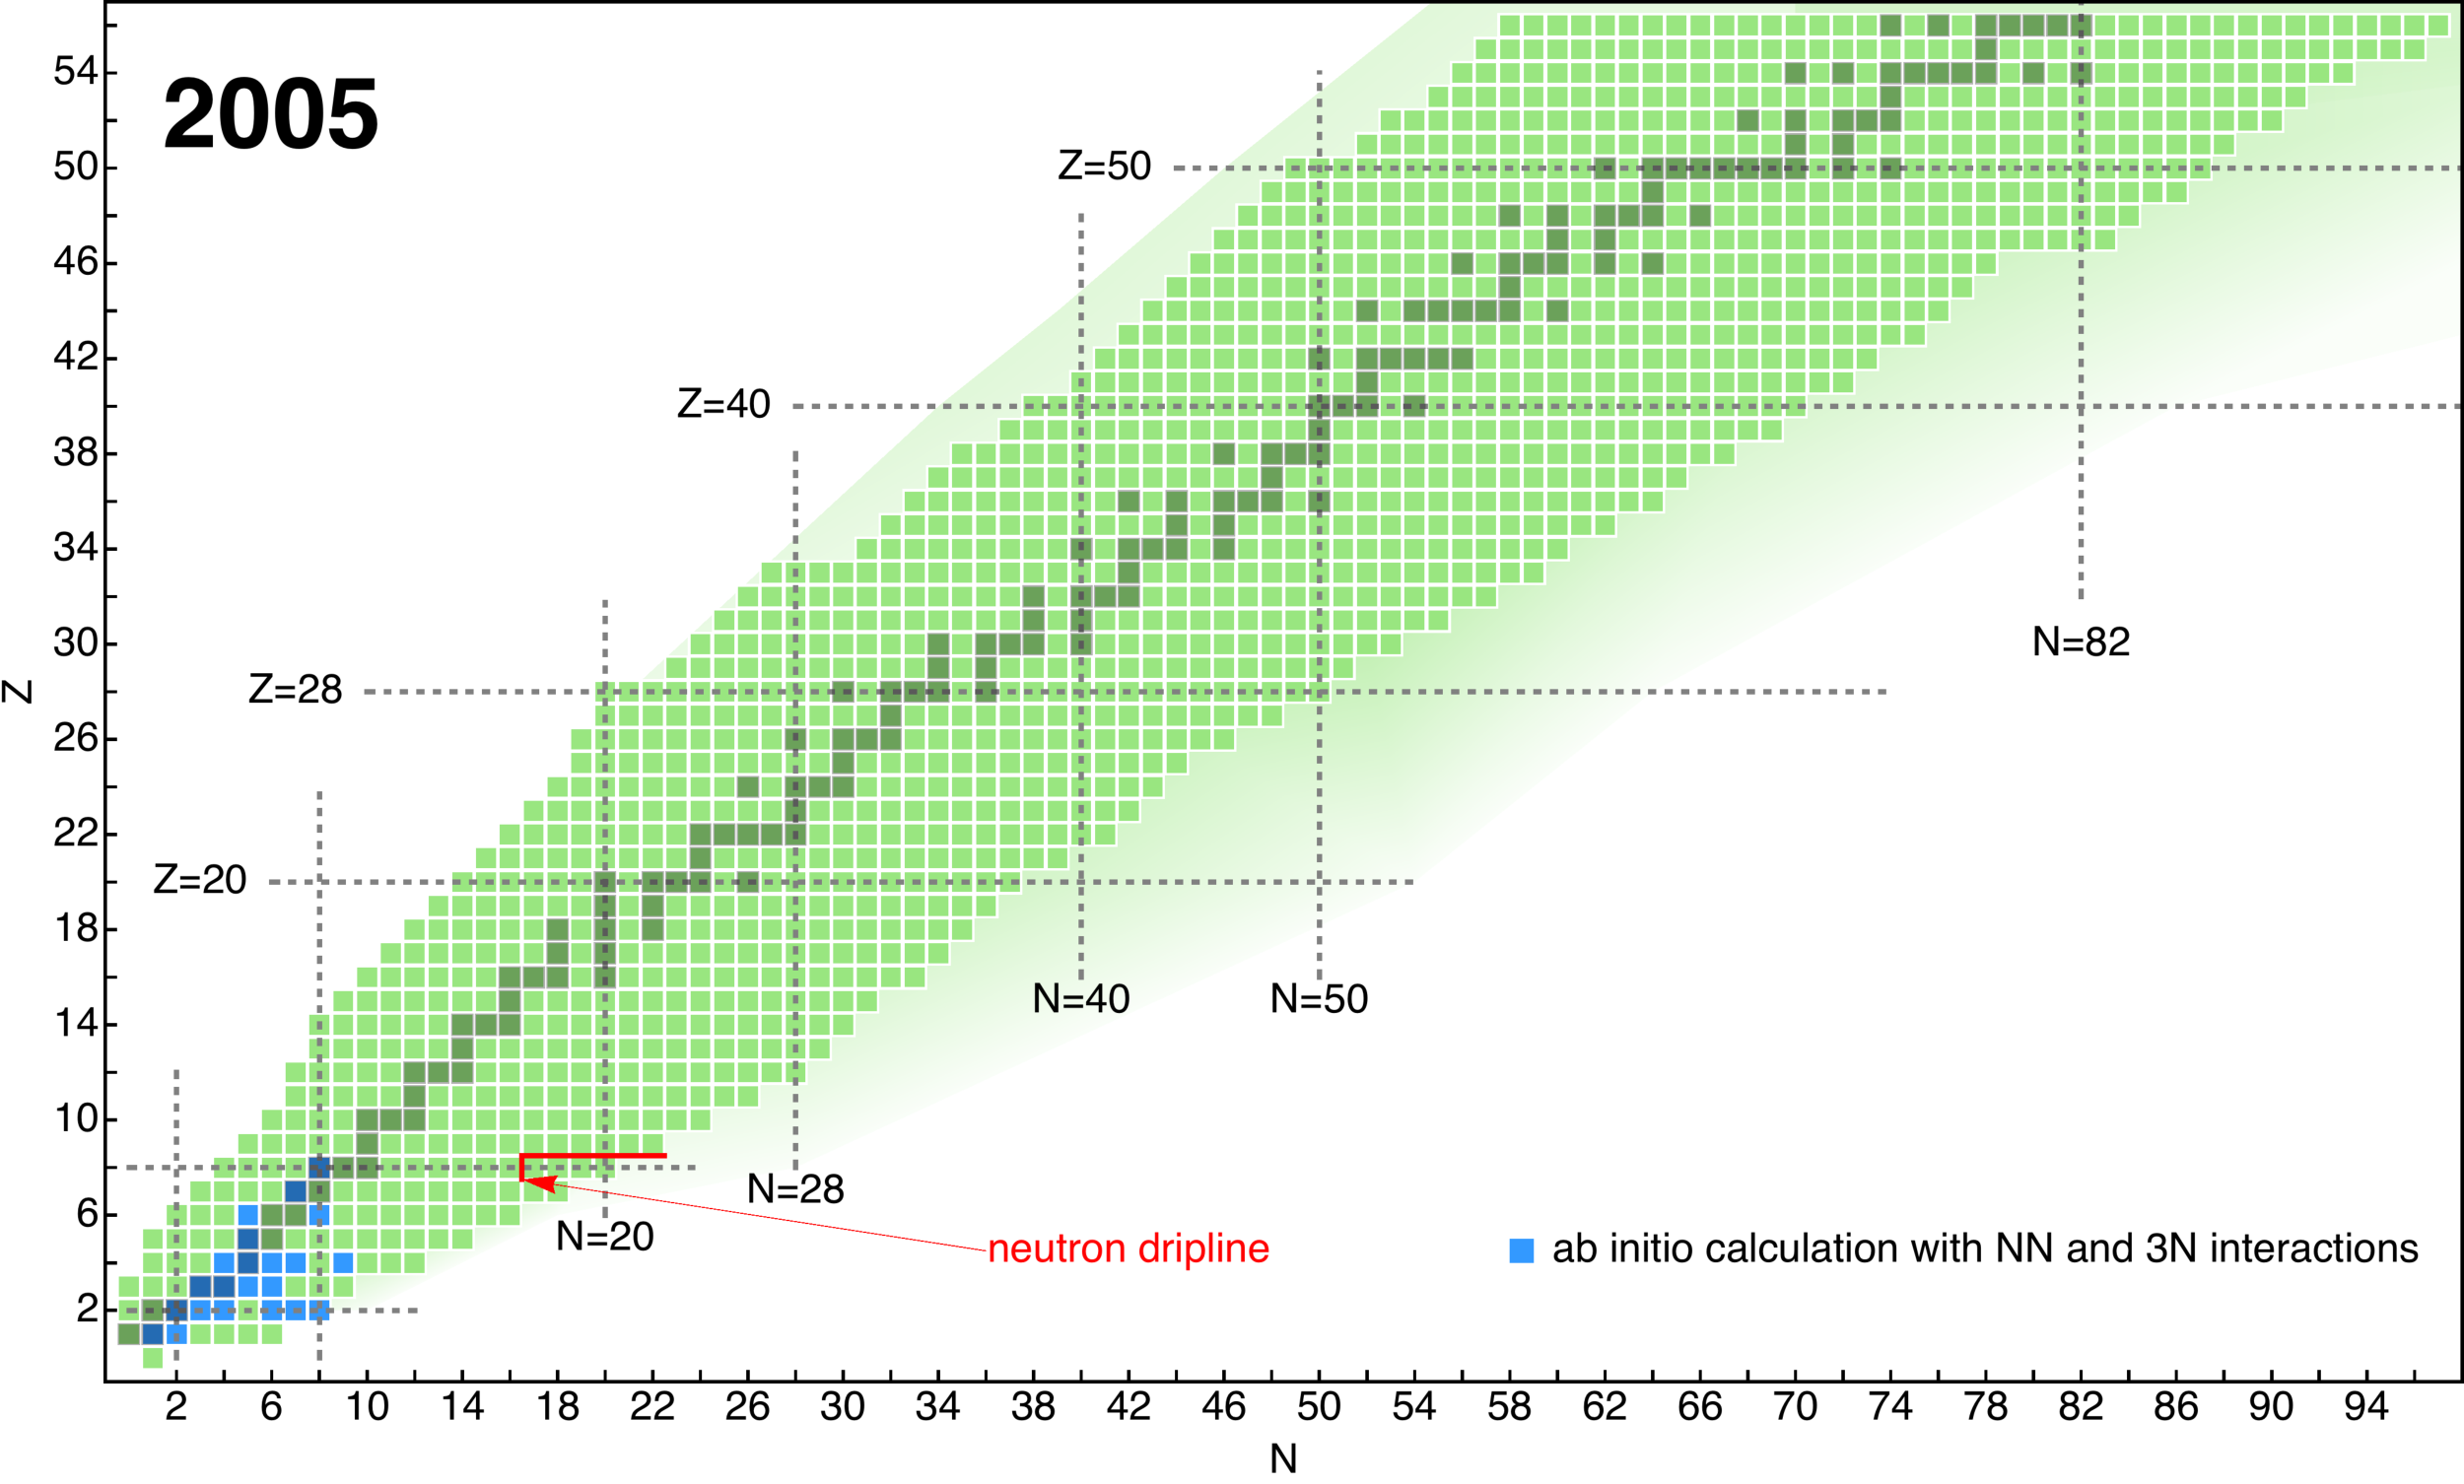
\includegraphics[trim={0 1.75cm 0 0},clip,width=0.7\linewidth]{nuclear_chart_2005}
        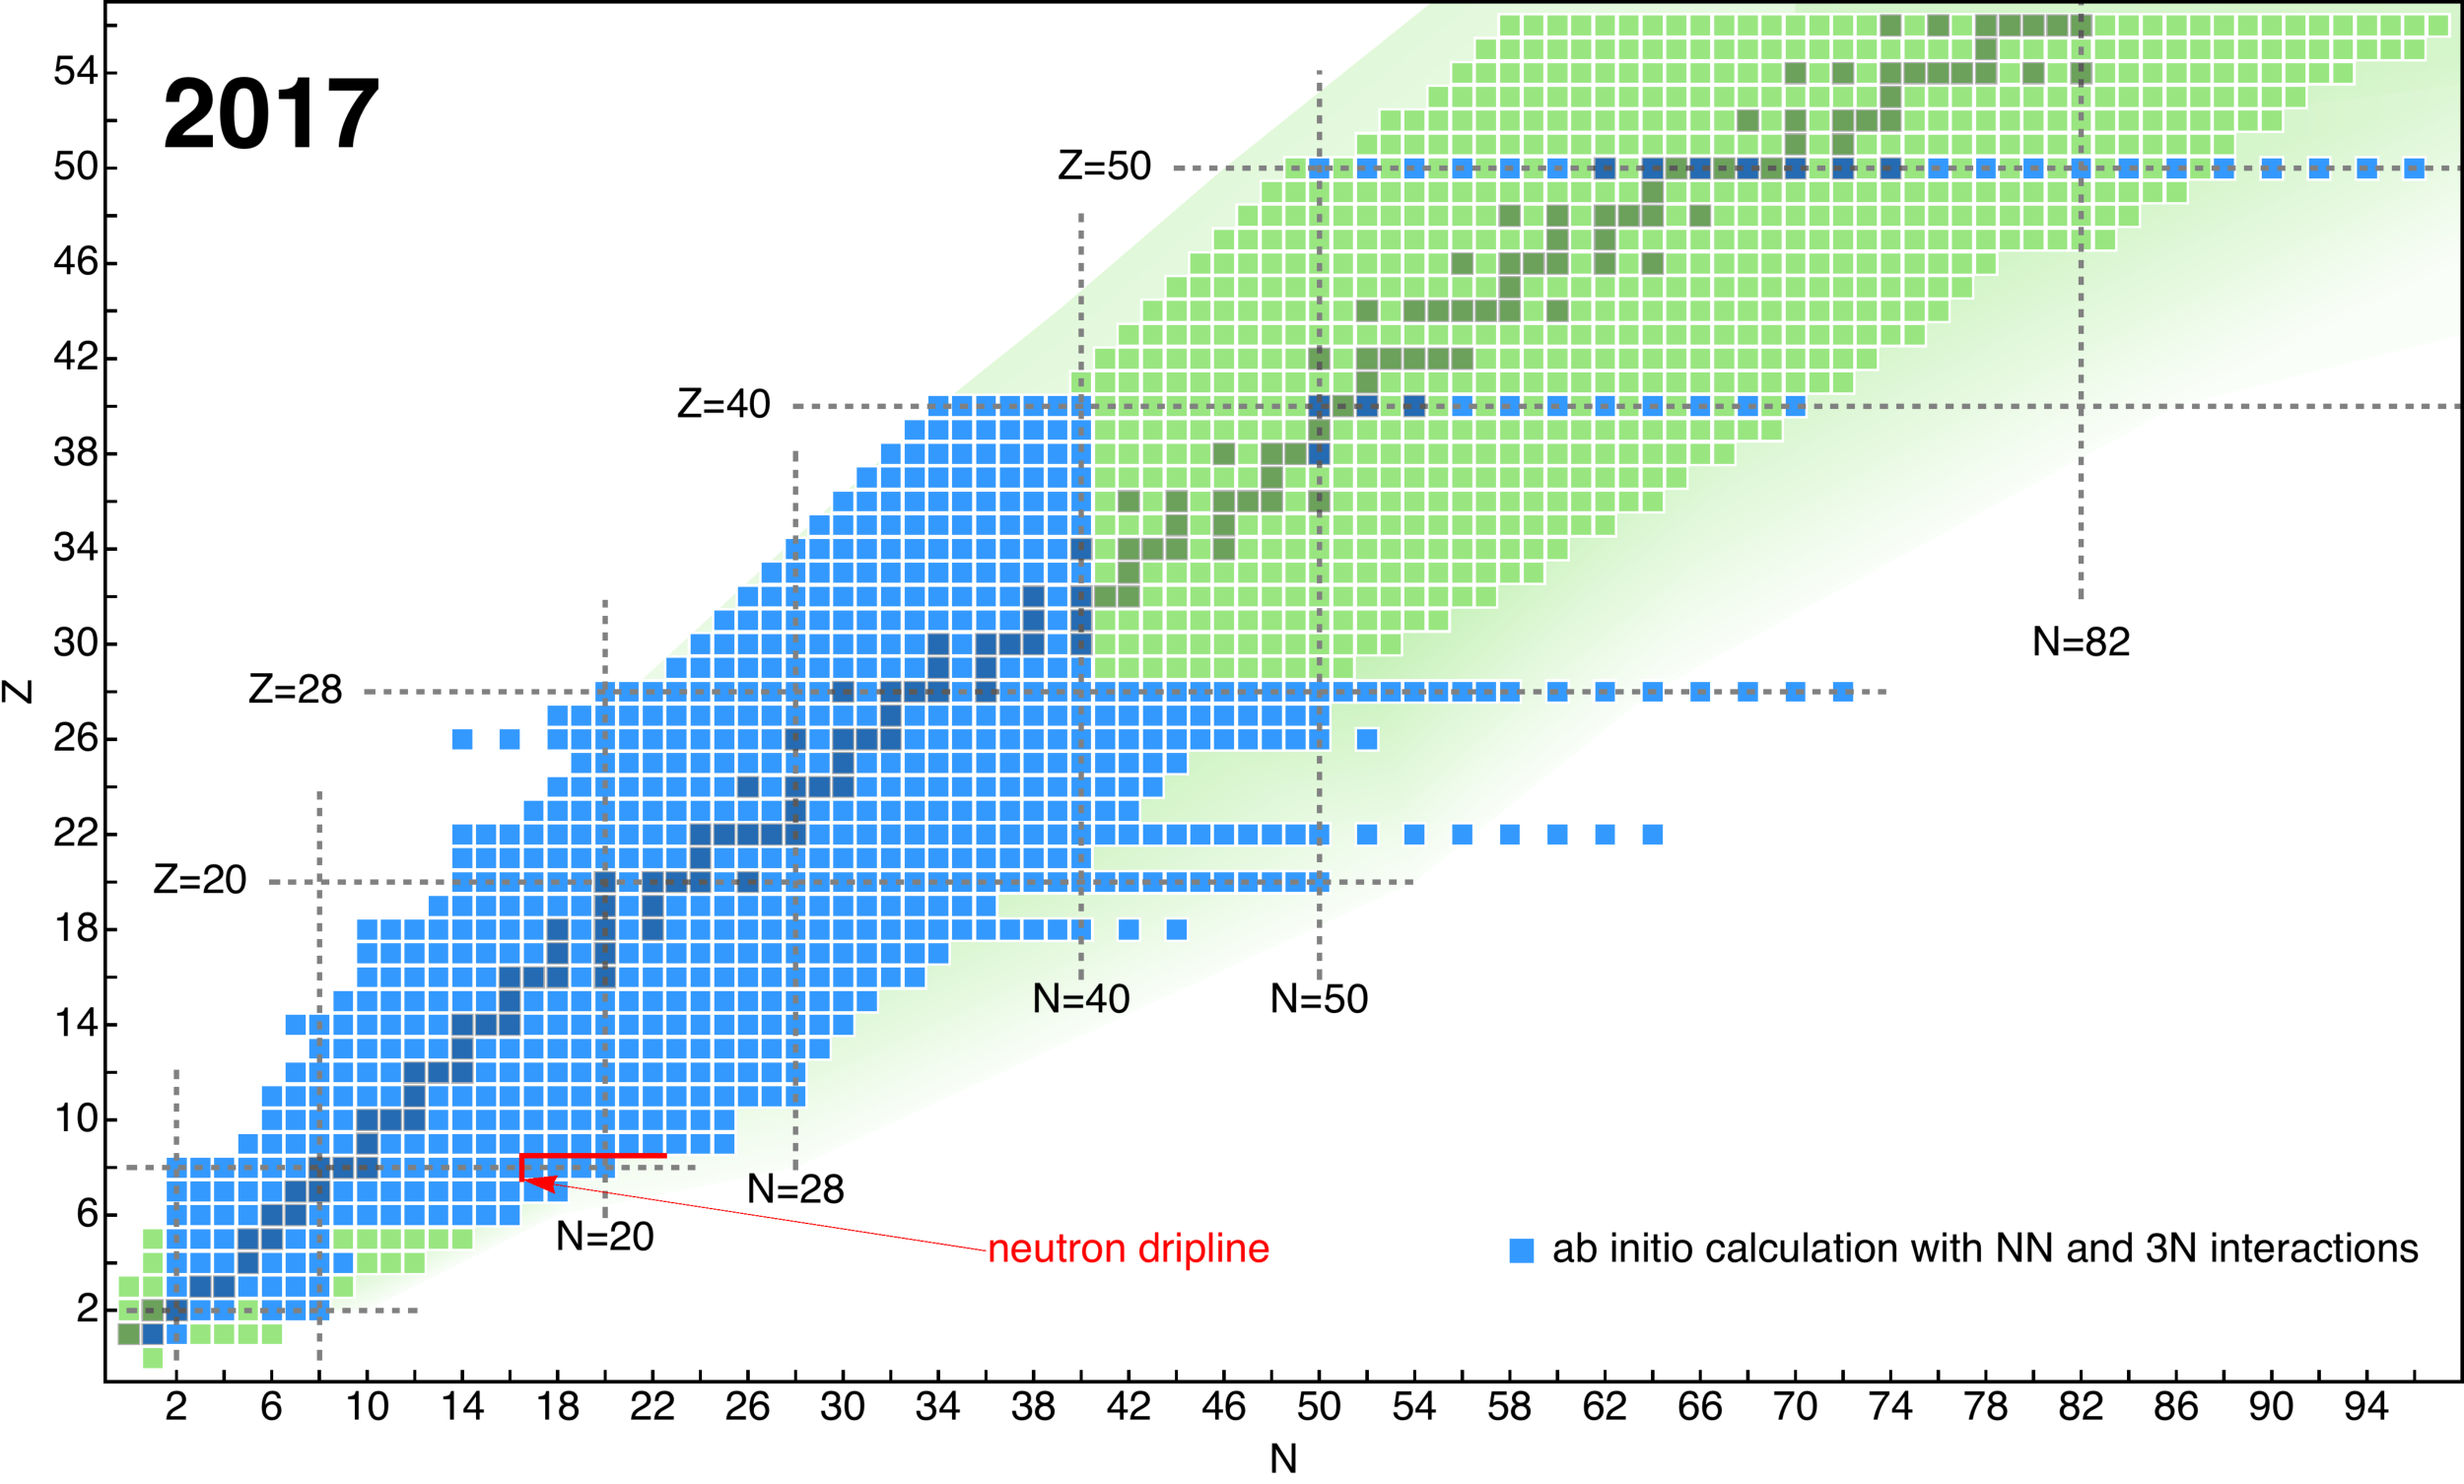
\includegraphics[width=0.7\linewidth]{nuclear_chart_2017}
    \end{center}
    \caption{Nuclear charts for 2005 and 2017 demonstrating the range of nuclei modeled using ab-initio methods. $Z$ and $N$ are proton and neutron number of the isotope, respectively.}
    \label{fig:nuclchart}
\end{figure}

In recent years, the improvements in computational hardware and the development of new computational methods has brought about a rapid expansion (see Fig.~\ref{fig:nuclchart}) in the range of nuclear isotopes able to be modeled via ab-initio calculations, which are calculations starting from the forces between nucleons as determined by scattering experiments and few-body nuclei. The improvements in computational hardware have come through the development and proliferation of high-throughput devices (such as GPUs) and the assembly of highly parallel systems. Current trends, shown in Fig.~\ref{fig:top500}, suggest that a machine with exa-FLOP (floating-point operations per second) throughput will exist by 2020 and such systems will be commonplace soon after \cite{Top500}. Much work is being done to ensure that the processing, networking, and power-consumption of these systems will continue to scale as it has for the past two decades.

\begin{figure}[t]
    \begin{center}
        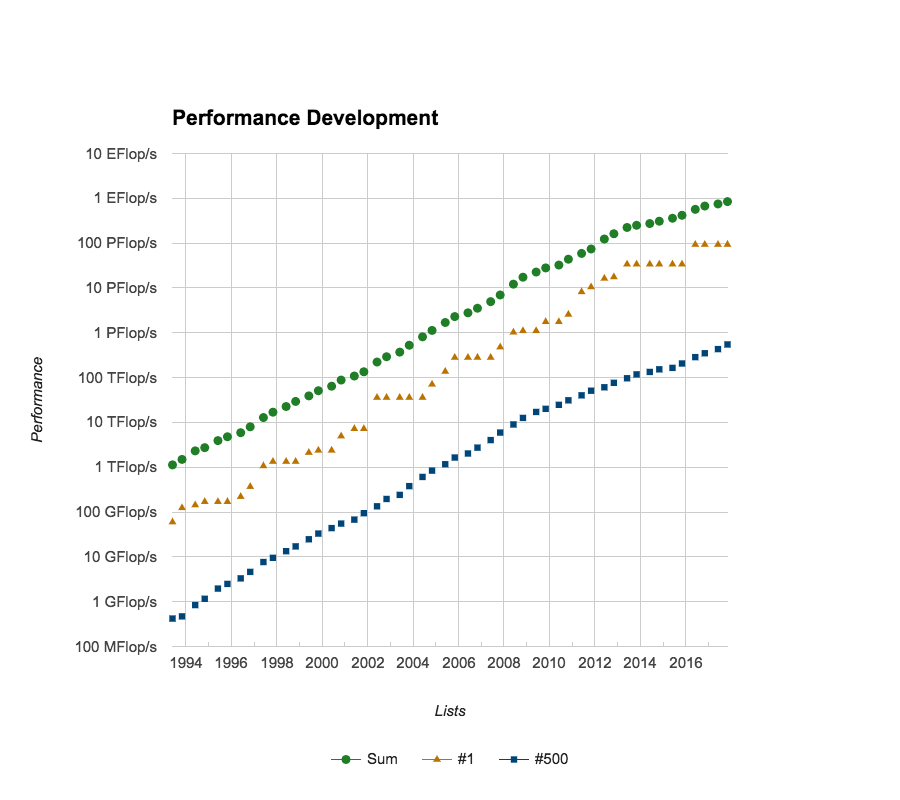
\includegraphics[trim={0 0 0 3.5cm},clip,width=0.8\linewidth]{top500}
    \end{center}
    \caption{According to the Top500 list of supercomputers, there should be an exa-scale cluster in 2020.}
    \label{fig:top500}
\end{figure}

The computational methods used in modern low-energy nuclear theory come in three classes: many-body methods, effective field theory (EFT) methods, and renormalization group (RG) methods. Modern many-body methods, like the no-core shell model (NCSM), seek to model nuclei from first principles and work in conjunction with RG and EFT methods to make these calculations feasible. EFT methods offer systematically improvable, model-independent expansions of nuclear interactions and other operators that allows for importance truncation and uncertainty quantification. RG methods are applied to interactions given by EFT methods and modify these interactions to match the resolution relevant to the problem at hand. These methods have already been used to provide both theoretical predictions that improve on previous calculations and theoretical predictions for nuclei that were unable to be modeled previously. The use of these methods in low-energy nuclear calculations is the state of the art. As a result, questions regarding their application are open problems and the focus of extensive research. % For low-energy nuclear physics, this means framing the problem in terms of low-energy nucleon-nucleon interactions, as opposed to the parton-parton interaction of the strong force. 

The similarity renormalization group method (SRG) is an interaction softening method from the class of RG methods whose use in nuclear theory was first explored in a 1-dimensional setting at OSU in 2007 \cite{Jurgenson:2007td}. It is a class of continuous unitary transformations that decouple large off-diagonal matrix elements in the interaction Hamiltonian, softening the potential as a result. The evolution of the Hamiltonian to a decoupled form allows a truncated subspace of the original basis to be used in later calculations without affecting the observables such as the energy eigenvalues. This basis truncation offers a significant reduction in the size of the problem. SRG is frequently used in modern nuclear theory calculations to soften interactions and extend the range of certain calculations to larger systems. In our work, we return to a simple 1-dimensional setting to study features of SRG and seek to understand how to optimize its use in many-body calculations.

\section{Contributions}

Our main contributions are:
\begin{itemize}
    \item{We have developed an open-source Python library with easy-to-use abstractions for the SRG method for use by others to test SRG in a simple setting.}
    \item{We verify the results published in the 2008 Jurgenson paper for 2-body and 3-body systems, validating our implementation for those systems and implying its correctness for general $A$-body systems. We also provide a suite of tests for the library, verifying that it fails gracefully when misused and correctly calculates the results of simple analytically solvable cases when used correctly.}
    \item{We explore some alternative transformation generators and seek to quantify their performance relative to the standard generator that is currently used. We discuss the results of these calculations and offer some preliminary analysis.}
\end{itemize}

\section{Outline}

The rest of the thesis is as follows:
\begin{itemize}
    \item{In chapter 2, we review the matrix representation of quantum operators. We then discuss the details of two different bases used, relative Jacobi momentum coordinates and 1-dimensional symmetrized harmonic oscillator states. We then discuss the details of the SRG method and explain the need for a careful revisit of SRG in a 1-dimensional setting.}
    \item{In chapter 3, we explain the design of the Python library. Much of the effort on this project went into making the library design logical and simple-to-use, so this chapter will explain the abstractions made and the reasoning behind those decisions.}
    \item{In chapter 4, we explain the approach taken to reproducing the 2008 Jurgenson results. We outline our approach to testing new transformation generators once our implementation has been validated.}
    \item{In chapter 5, we present our results. We discuss in detail the various different ways in which we verify that what we are doing is correct at each stage of the exploration. Finally, we show some alternative transformation generators that induce smaller 3-body forces.}
    \item{In chapter 6, we summarize our results, point to open questions and specific points of interest, and discuss what features of the \texttt{srg1d} library still need to be implemented.}
\end{itemize}

